% !TeX root = ../regression_logistique.tex
\chapter{Surface de perte et longueur du pas}
\label{ann:optimisation}

\orient{%
lire une descente sur la surface de perte et sur ses lignes de niveau ; relier
la longueur du pas à la courbure de la perte ; énoncer la condition suffisante de
décroissance}{%
dérivée partielle et gradient (\annexeref{ann:prerequis}) ;
chapitre~\ref{ch:descente} ; \annexeref{ann:convexite}}{%
approfondissement}

\textbf{Résultat employé dans le fil principal.} Le réglage $\alpha=1$ retenu au
chapitre~\ref{ch:descente} fait décroître la perte à chaque tour. Cette annexe
donne la condition qui l'assure, la borne qui la quantifie, et la lecture
géométrique de la trajectoire.

\section{Surface du coût}

Chaque couple de coefficients produit un coût, calculable sur les $1\,600$
observations. Porter ce coût en altitude au-dessus du couple qui le produit
définit une surface au-dessus du plan $(w_1,w_2)$, dont chaque point représente
un modèle possible. Le coût dépendant de trois coefficients, sa représentation
demanderait quatre dimensions ; fixer le biais à sa valeur finale ramène à deux.

Cette surface est convexe (\annexeref{ann:convexite}), donc sans minimum local
parasite, et sa pente décroît à l'approche du minimum, ce qui raccourcit les pas
successifs.

\begin{figure}[htbp]
\centering
\begin{graphique}{Courbe décroissante de la longueur du gradient en échelle logarithmique, de 0,42 à 0,0026 sur 400 itérations, sans plateau.}
\begin{tikzpicture}
\begin{axis}[courseplot,height=5.6cm,axis lines=left,ymode=log,
  xlabel={itération},ylabel={longueur du gradient},xmin=0,xmax=400]
  \addplot[warning,very thick,no markers] table[x=iter,y=norm] {data/gradient.dat};
\end{axis}
\end{tikzpicture}
\end{graphique}
\caption{Longueur du gradient en échelle logarithmique, de $0{,}42$ à
$0{,}0026$ en $400$ itérations. Cette décroissance fournit le critère d'arrêt.}
\label{fig:ann-opt-norme-gradient}
\end{figure}

La descente se lit sur la surface : partant d'un point, elle suit la direction
opposée au gradient et progresse par pas de longueur proportionnelle à $\alpha$.
Le gradient étant orthogonal aux lignes de niveau, la trajectoire les coupe
perpendiculairement.

Les deux figures suivantes tracent une descente à \emph{deux} coefficients, le
biais restant figé à $w_0=-4{,}745$ tandis que $w_1$ et $w_2$ se déplacent. Elle
est réellement exécutée sur la surface affichée, ce qui rend cette lecture
exacte, et se distingue sur deux points de la descente à trois coefficients du
chapitre~\ref{ch:descente}. Son point de départ $(0\,;0)$ vaut $J=0{,}98$ plutôt
que $\log 2=0{,}693$, le biais n'y étant pas nul ; et le minimum qu'elle atteint,
$(-3{,}489\,;+3{,}512)$, est le meilleur couple \emph{sous la contrainte} d'un
biais figé, légèrement distinct de \Mquatre.

\begin{figure}[htbp]
\centering
\makebox[\textwidth][c]{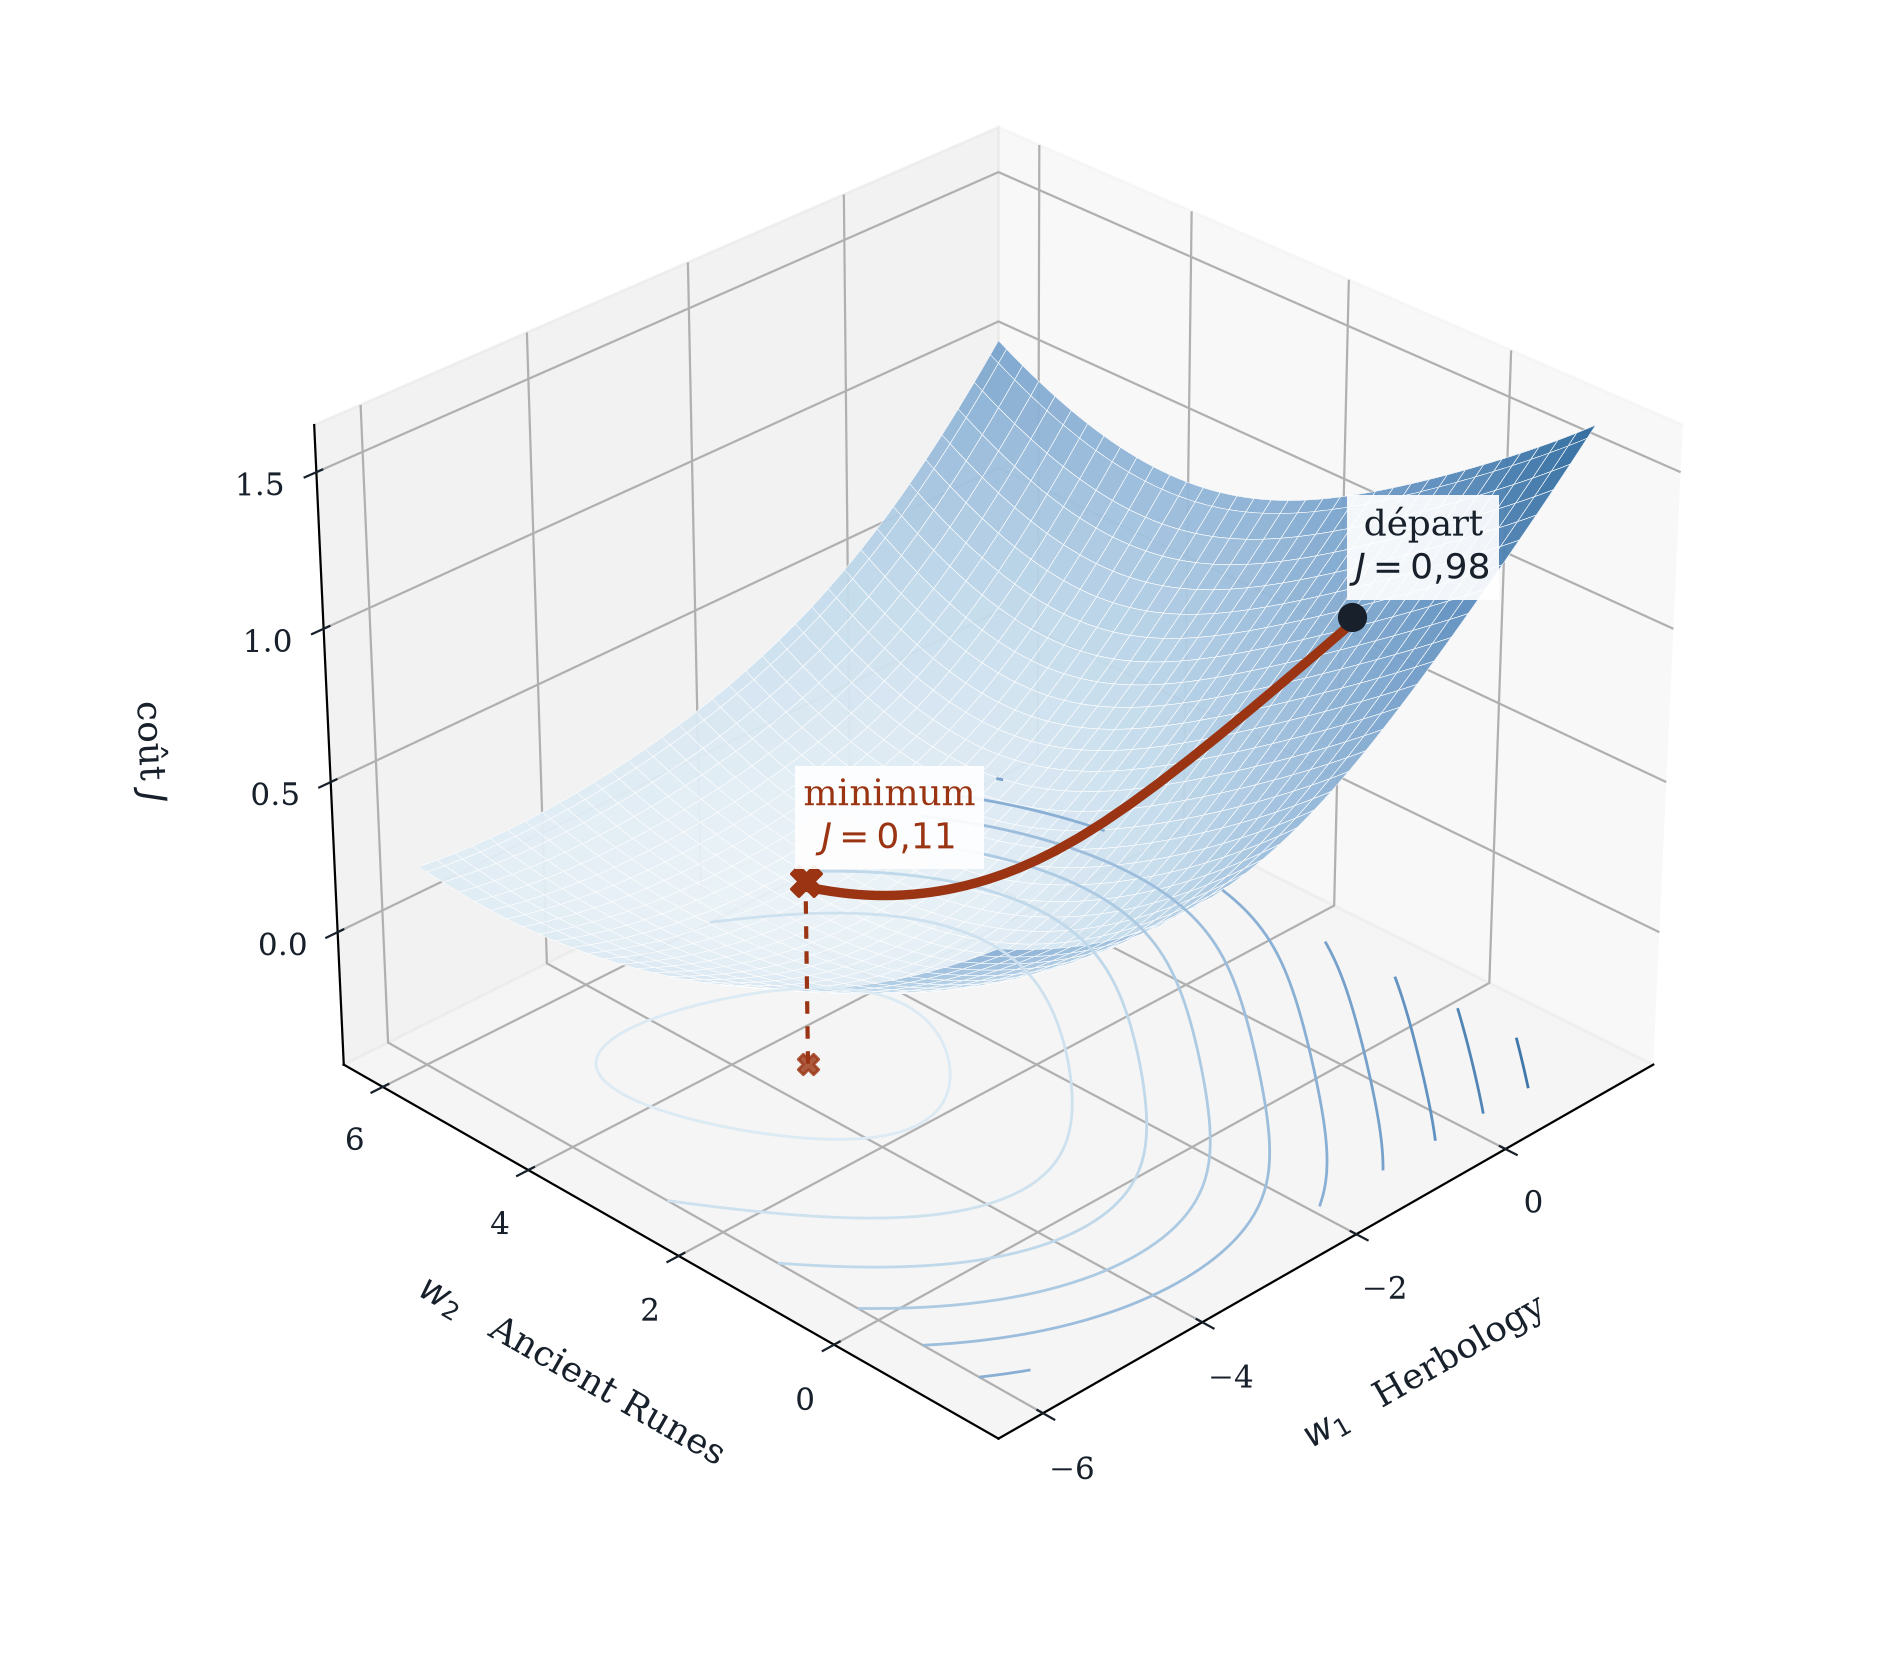
\includegraphics[width=\textwidth,
  alt={Surface tridimensionnelle de la perte moyenne au-dessus du plan des coefficients w1 et w2, en forme de cuvette allongée. Une courbe rouge descend du bord vers le fond, de 0,98 à 0,11, en coupant les lignes de niveau tracées au sol.}]{figures/surface3d.png}}
\caption{Surface de perte au-dessus du plan $(w_1,w_2)$, biais figé à
$w_0=-4{,}745$. La courbe rouge est une descente à deux coefficients exécutée
sur cette surface, de $J=0{,}98$ à $J=0{,}11$.}
\label{fig:ann-opt-surface}
\end{figure}

\begin{figure}[htbp]
\centering
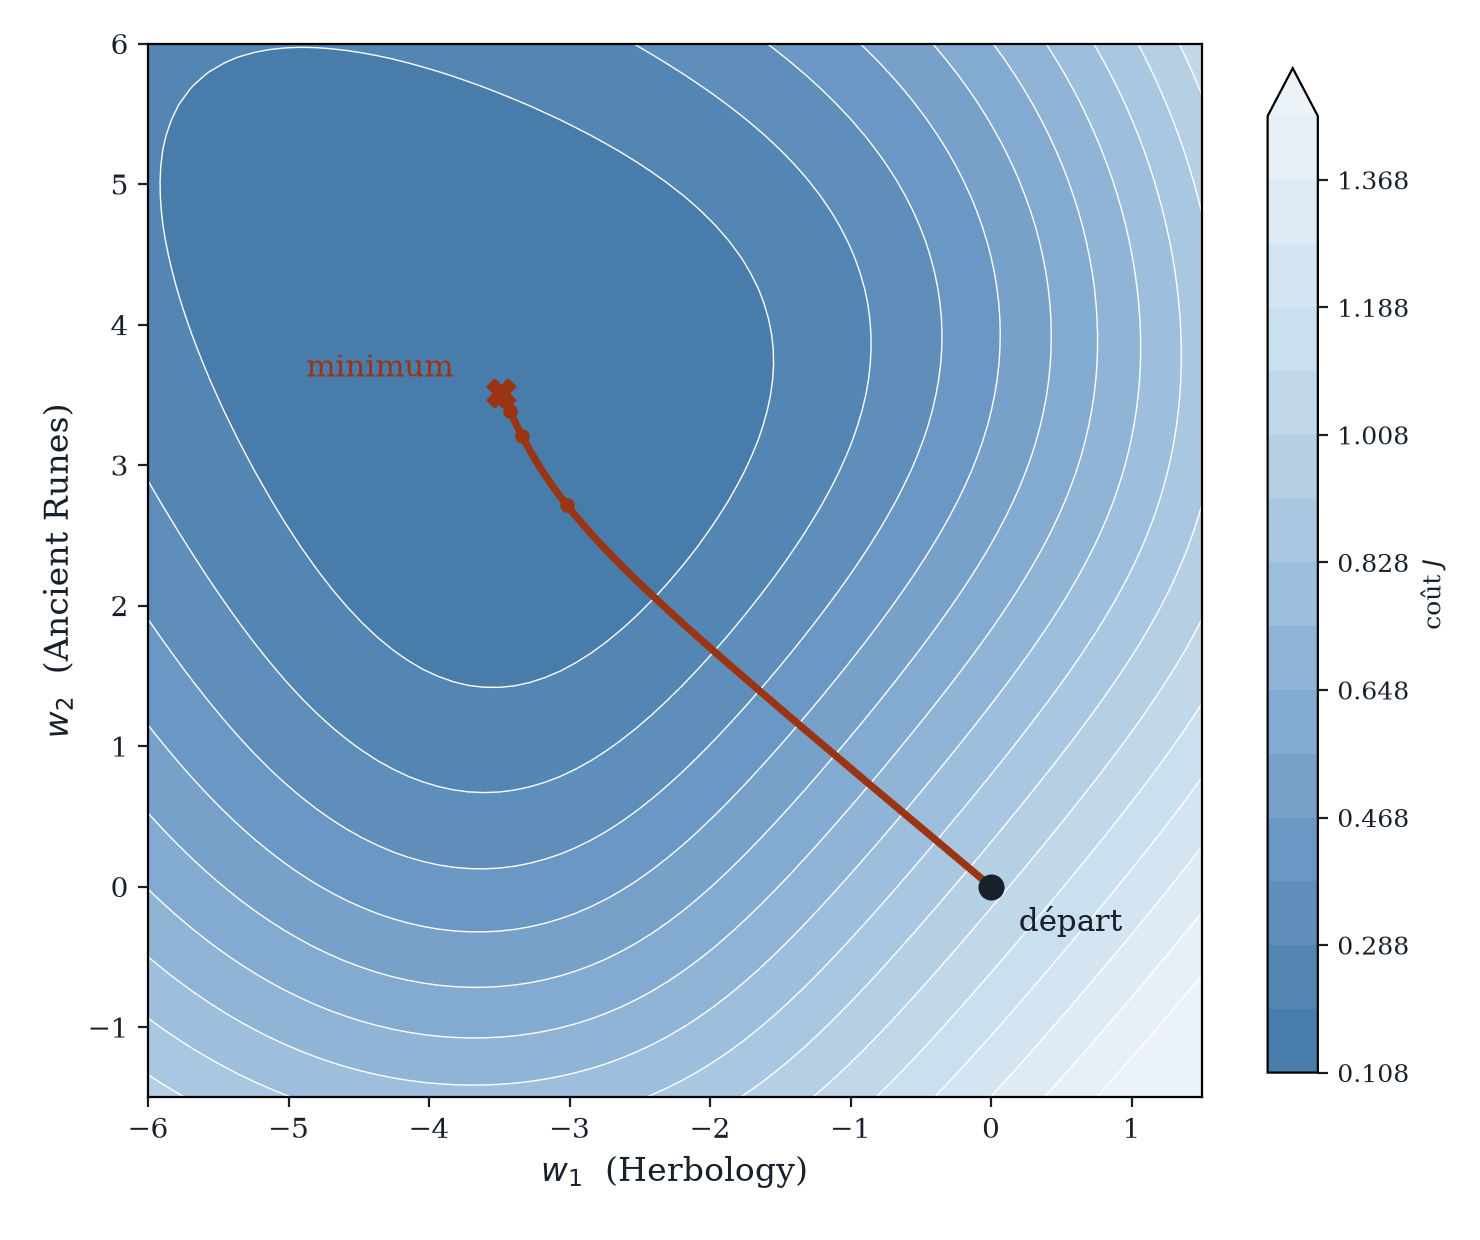
\includegraphics[width=.78\textwidth,
  alt={Lignes de niveau de la perte dans le plan des coefficients, en ellipses emboîtées. La trajectoire de descente les coupe perpendiculairement ; ses points, marqués toutes les vingt-cinq itérations, s'espacent au début et se resserrent près du fond.}]{figures/contours.png}
\caption{La même surface vue de dessus. Chaque courbe relie les couples de perte
égale ; la trajectoire les coupe perpendiculairement. Les points marquent une
itération sur vingt-cinq.}
\label{fig:ann-opt-contours}
\end{figure}
\FloatBarrier

\section{Longueur du pas}

À chaque tour, le gradient fournit une direction : son opposé $-\nabla J$ est
celle dans laquelle la perte décroît le plus vite depuis le point courant. La
distance à parcourir dans cette direction est fixée par $\alpha$. Direction et
longueur sont deux décisions séparées : la première se calcule, la seconde se
règle.

Un pas court consomme la correction disponible par fractions, et il en faut
d'autant plus de tours pour parcourir la même distance. Chaque tour demandant un
passage complet sur les $1\,600$ lignes, ce choix se paie en temps de calcul pour
aboutir à la même frontière.

Un pas long expose au dépassement. La pente que donne le gradient décrit
fidèlement le terrain au seul voisinage du point où elle est calculée. Sortir de
ce voisinage fait passer les coefficients de l'autre côté du minimum, sur la
pente opposée, et le coût augmente. Les tours suivants ramènent vers le bas, au
prix d'un détour.

\begin{figure}[htbp]
\centering
\begin{graphique}{Quatre courbes de coût sur quarante itérations. Le pas 0,05 décroît lentement et reste très au-dessus. Les pas 0,3 et 1 décroissent régulièrement. Le pas 100 descend d'abord plus vite puis présente une trajectoire heurtée avant de rejoindre le bas.}
\begin{tikzpicture}
\begin{axis}[width=.82\textwidth,height=6.8cm,
  axis lines=left,axis line style={ink!40},
  grid=major,grid style={gridgray!30},
  tick label style={font=\small},label style={font=\small},
  xlabel={itération},ylabel={coût $J$},
  xmin=0,xmax=40,ymin=0.09,ymax=0.72,
  legend style={at={(0.98,0.97)},anchor=north east,draw=none,font=\small,
    fill=white,fill opacity=0.85,text opacity=1}]
  \addplot[warning,very thick,no markers] table[x=iter,y=a005] {data/alpha.dat};
  \addlegendentry{$\alpha=0{,}05$}
  \addplot[huffle,thick,densely dashed,no markers]
    table[x=iter,y=a03] {data/alpha.dat};
  \addlegendentry{$\alpha=0{,}3$}
  \addplot[accent,very thick,no markers] table[x=iter,y=a10] {data/alpha.dat};
  \addlegendentry{$\alpha=1$}
  \addplot[slyth,thick,densely dotted,no markers]
    table[x=iter,y=a1000] {data/alpha.dat};
  \addlegendentry{$\alpha=100$}
\end{axis}
\end{tikzpicture}
\end{graphique}
\caption{Quarante itérations à partir de \Mzero, quatre réglages du pas. À
$\alpha=100$, la trajectoire est heurtée : le déplacement dépasse le minimum le
long de plusieurs directions.}
\label{fig:ann-opt-alpha-reel}
\end{figure}
\FloatBarrier

\begin{chiffres}[Perte moyenne selon le pas]
\begin{center}
\begin{tabular}{crrrl}
\toprule
$\alpha$ & départ & après un tour & après quarante & \\
\midrule
$0{,}05$ & $0{,}693147$ & $0{,}684362$ & $0{,}466848$ & pas trop court \\
$0{,}3$  & $0{,}693147$ & $0{,}642124$ & $0{,}237761$ & \\
$1$      & $0{,}693147$ & $0{,}538507$ & $0{,}153427$ & réglage retenu \\
$100$    & $0{,}693147$ & $0{,}408290$ & $0{,}111846$ & trajectoire heurtée \\
$1\,000$ & $0{,}693147$ & $4{,}049$    & --- & premier pas au-delà de la cible \\
\bottomrule
\end{tabular}
\end{center}
Les cinq réglages partent de $\log 2$, les coefficients nuls donnant $0{,}5$
partout. À $\alpha=100$, le faible gradient initial produit encore une baisse
au premier tour malgré l'amplitude du déplacement ; la trajectoire devient
ensuite heurtée. À $\alpha=1\,000$, le premier tour porte
la perte de $0{,}69$ à $4{,}05$. Le seuil se lit sur la courbe, non à l'{\oe}il.
\end{chiffres}

$\alpha$ se règle par essais, en lisant la courbe de perte : un bon réglage la
fait décroître à chaque tour, vite d'abord puis de moins en moins. Une remontée,
même isolée, indique un pas trop long. Le cours retient $\alpha=1$.

\section{Condition de décroissance}

La longueur du déplacement, $\alpha\|\nabla J\|$, croît sans borne avec $\alpha$,
et un pas suffisamment grand fait diverger la descente. Le seuil au-delà duquel
cela se produit est fixé par la courbure de $J$ par rapport aux
\emph{coefficients}, c'est-à-dire par la hessienne
$\tfrac{1}{m}\X^{\!\top}S\X$, qui fait intervenir l'échelle et les corrélations
des colonnes de $\X$ (\annexeref{ann:convexite}). La borne $p(1-p)\leq\frac14$
porte sur le seul facteur $s_i$ et laisse ce seuil indéterminé.

L'énoncé exact est conditionnel. Si le gradient de $J$ est $L$-lipschitzien ---
ce qui est le cas ici, avec $L\leq\tfrac{1}{4m}\|\X\|^2$ --- alors tout pas
$\alpha<2/L$ fait décroître $J$ à chaque tour, et $\alpha\leq1/L$ garantit une
convergence en $O(1/t)$~\cite{nocedal2006,boyd2004}. Ce seuil dépend des données,
d'où le réglage par essais plutôt que par formule.

La standardisation des colonnes (ch.~\ref{ch:standardisation}) intervient
directement : en rapprochant les échelles des colonnes, elle réduit l'écart entre
les courbures dans les différentes directions et rend un même $\alpha$ acceptable
pour tous les coefficients.

\begin{figure}[htbp]
\centering
\begin{graphique}{Deux graphiques de suites d'itérés d'une quadratique de minimum 2, ligne pointillée horizontale. À gauche, pas adapté : les points convergent vers 2 en se rapprochant à chaque tour. À droite, pas critique : les points oscillent indéfiniment entre -2 et 6.}
\begin{minipage}[t]{.48\textwidth}
\centering
\begin{tikzpicture}[alt={Suite d'itérés d'une fonction quadratique avec un pas adapté ; les points convergent vers le minimum situé en 2.}]
\begin{axis}[width=.95\linewidth,height=5.4cm,axis lines=left,
  title={$\alpha$ adapté},xlabel={itération},ylabel={$\theta$},
  xmin=0,xmax=6,ymin=-2.6,ymax=6.6,grid=major,grid style={gridgray!45}]
  \addplot[accent,very thick,mark=*] coordinates
    {(0,-2) (1,0) (2,1) (3,1.5) (4,1.75) (5,1.875) (6,1.9375)};
  \addplot[ink,dashed,thick,domain=0:6]{2};
\end{axis}
\end{tikzpicture}
\end{minipage}\hfill
\begin{minipage}[t]{.48\textwidth}
\centering
\begin{tikzpicture}[alt={Suite d'itérés de la même fonction avec le pas critique ; les points oscillent entre -2 et 6 sans converger vers le minimum situé en 2.}]
\begin{axis}[width=.95\linewidth,height=5.4cm,axis lines=left,
  title={$\alpha$ trop grand},xlabel={itération},ylabel={$\theta$},
  xmin=0,xmax=6,ymin=-2.6,ymax=6.6,grid=major,grid style={gridgray!45}]
  \addplot[warning,very thick,mark=*] coordinates
    {(0,-2) (1,6) (2,-2) (3,6) (4,-2) (5,6) (6,-2)};
  \addplot[ink,dashed,thick,domain=0:6]{2};
\end{axis}
\end{tikzpicture}
\end{minipage}
\end{graphique}
\caption{Quadratique d'une variable, courbure $c$, minimum en $2$. À gauche
$\alpha<2/c$ : convergence. À droite $\alpha=2/c$ : oscillation entre deux
valeurs ; tout $\alpha>2/c$ diverge.}
\label{fig:ann-opt-alpha-quadratique}
\end{figure}
\FloatBarrier

\begin{exercice}[Pas critique d'une quadratique]
Soit $f(\theta)=\tfrac{c}{2}(\theta-2)^2$ avec $c=4$. Écrire l'itération de
descente de gradient, en déduire la relation entre $\theta_{t+1}-2$ et
$\theta_t-2$, puis la valeur de $\alpha$ à partir de laquelle la suite cesse de
converger. Vérifier sur la
figure~\ref{fig:ann-opt-alpha-quadratique}.
\end{exercice}

\textbf{Retour au fil principal.} Le critère d'arrêt et les régimes successifs de
la descente sont au chapitre~\ref{ch:descente}, section~5.
